\documentclass[margin=0.2cm]{standalone}
\usepackage{amsmath}
\usepackage{amssymb}
\usepackage{tikz}
\usetikzlibrary{shapes, arrows.meta}
\begin{document}
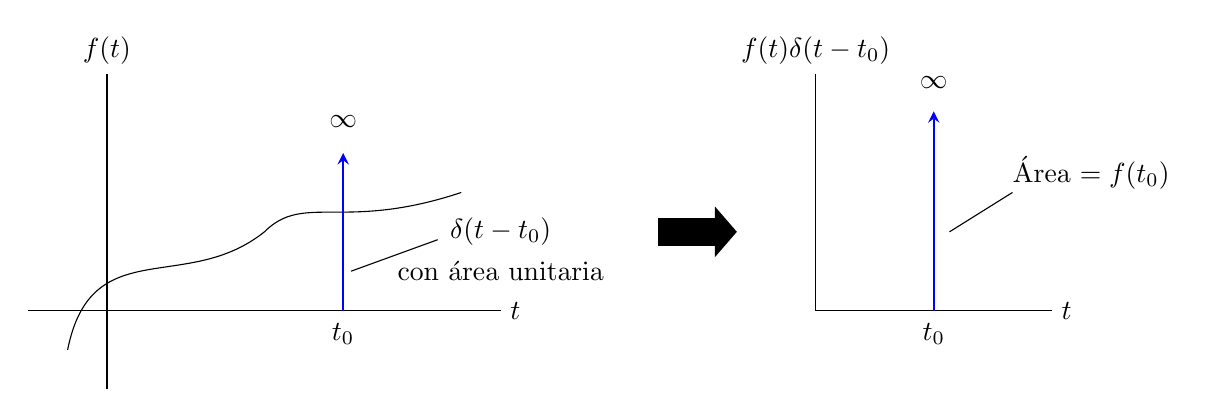
\begin{tikzpicture}
	\draw (-1, 0) -- (5, 0) node[right] {$t$};
	\draw (0, -1) -- (0, 3) node[above] {$f(t)$};

    \draw (-0.5, -0.5) .. controls (-0.2, 1) and (1, 0.2) .. (2, 1) .. controls (2.5, 1.5) and (3, 1) .. (4.5, 1.5);

    \draw[blue, -stealth, thick] (3, 0) -- (3, 2);
    \node at (3, -0.3) {$t_{0}$};
    \node at (3, 2.4) {$\infty$};
    \node at (5, 1) {$\delta (t - t_{0})$};
    \node at (5, 0.5) {con área unitaria};
    \draw (4.2, 0.9) -- (3.1, 0.5);

    \draw[-{Triangle[width=18pt,length=8pt]}, line width=10pt] (7, 1) -- (8, 1);

    \draw (9, 0) -- (12, 0) node[right] {$t$};
	\draw (9, 0) -- (9, 3) node[above] {$f(t) \delta(t - t_{0})$};

    \draw[blue, -stealth, thick] (10.5, 0) -- (10.5, 2.53);
    \node at (10.5, 2.9) {$\infty$};
    \node at (10.5, -0.3) {$t_{0}$};
    \node at (12.5, 1.75) {Área $= f(t_{0})$};
    \draw (11.5, 1.5) -- (10.7, 1);
\end{tikzpicture}
\end{document}